
% This LaTeX was auto-generated from MATLAB code.
% To make changes, update the MATLAB code and republish this document.

\documentclass{article}
\usepackage{graphicx}
\usepackage{color}

\sloppy
\definecolor{lightgray}{gray}{0.5}
\setlength{\parindent}{0pt}

\begin{document}

    
    

\section*{15. Lebesgue constants}

\begin{verbatim}
ATAPformats
\end{verbatim}
\begin{par}
There is a well developed theory that quantifies the convergence or divergence of polynomial interpolants.  A key notion is that of the \textit{Lebesgue constant,} $\Lambda$, for interpolation in a given set of points.  The Lebesgue constant is the $\infty$-norm of the linear mapping from data to interpolant: $$ \Lambda = \sup_{f} {\|p\|\over \|f\|}, \eqno (15.1) $$ where $\|\cdot\|$ denotes the $\infty$-norm in $C([-1,1])$.  In words, if you have data values on an $(n+1)$-point grid, and the data come from sampling a function that is no greater than 1 in absolute value, what is the largest possible value of the interpolant $p$ somewhere in $[-1,1]$?
\end{par} \vspace{1em}
\begin{par}
In the plots of Chapter 13 for interpolation of Runge's function, for example, we saw that the interpolants grew much bigger than the data. Thus the Lebesgue constants must be large for equispaced interpolation. For example, for $n=50$, the data are bounded by 1 for all $n$, yet the interpolant is bigger than $10^5$.  Thus the Lebesgue constant for interpolation in 50 equispaced points must be greater than $10^5$.  (In fact, it is about $4.2\times 10^{12}$.)
\end{par} \vspace{1em}
\begin{par}
From the basic Lagrange formula (5.1) for polynomial interpolation, $$ p(x) = \sum_{j=0}^n f_j \kern 1pt \ell_j(x), \eqno (15.2) $$ we can get a formula for $\Lambda$ in terms of the Lagrange polynomials $\{\ell_j\}$. At any point $x\in [-1,1]$, the maximum possible value of $|\kern .5pt p(x)|$ for grid data bounded by 1 in absolute value will be the number $\lambda(x)$ obtained if each data value is $\pm 1$, with signs chosen to make all the signs at $x$ coincide: $$ \lambda(x) = \sum_{j=0}^n |\ell_j(x)|. \eqno (15.3) $$ This sum of absolute values is known as the \textit{Lebesgue function} for the given grid, and the Lebesgue constant is equal to its maximum value, $$ \Lambda = \sup_{x\in[-1,1]} \lambda(x). \eqno (15.4) $$
\end{par} \vspace{1em}
\begin{par}
The reason Lebesgue constants are interesting is that interpolants are guaranteed to be good if and only if the Lebesgue constants are small. We can make this statement precise as follows. Let $\Lambda$ be the Lebesgue constant for interpolation in a certain set of points.  Without loss of generality (since the interpolation process is linear), suppose the largest absolute value of the samples is 1.  If $p$ is the interpolant in these points to a function $f$, we know that $\|p\|$ might be as great as $\Lambda$; yet $\|f\|$ might be as small as 1.  Thus $\|f-p\|$ might be as great as $\Lambda-1$, showing that a large Lebesgue constant rigorously implies the possibility of a large interpolation error.
\end{par} \vspace{1em}
\begin{par}
Conversely, let $p^*$ be the best degree $n$ polynomial approximation to $f$ in the $\infty$-norm. If $p$ is the polynomial interpolant to $f$ in the given points, then $p-p^*$ is the polynomial interpolant to $f-p^*$. By the definition of the Lebesgue constant, $\|\kern .7pt p-p^*\|$ is no greater than $\Lambda \|f-p^*\|$.  Since $f-p = (f-p^*)-(\kern .7pt p-p^*)$, this implies that $\|f-p\|$ is no greater than $(\Lambda+1)\|f-p^*\|$.  Thus a small Lebesgue constant implies that interpolation will be close to best.
\end{par} \vspace{1em}
\begin{par}
Actually, the discussion of the last two paragraphs is not limited to interpolation.  What is really in play here is any approximation process that is a \textit{linear projection} from $C([-1,1])$ to ${\cal P}_n$, of which Chebyshev projection (truncation of the Chebyshev series) would be an example as well as interpolation. Suppose we let $L$ denote an operator that maps functions $f\in C([-1,1])$ to approximations by polynomials $p\in {\cal P}_n$.  For $L$ to be linear means that $L(f_1+f_2) = L f_1 + Lf_2$ for any $f_1, f_2 \in C([-1,1])$ and $L(\alpha f) = \alpha Lf$ for any scalar $\alpha$, and for $L$ to be a projection means that if $p\in {\cal P}_n$, then $Lp = p$. By the argument above we have established the following result applicable to any linear projection.
\end{par} \vspace{1em}
\begin{par}
 \em
{\bf Theorem 15.1. Near-best approximation and Lebesgue constants.} Let
$\Lambda$ be the Lebesgue constant for a linear projection $L$ of
$C([-1,1])$ onto ${\cal P}_n$.  Let $f$ be a function in $C([-1,1])$, $p =
Lf$ the corresponding polynomial approximant to $f$, and $p^*$ the best
approximation.  Then
$$ \|f-p\| \le (\Lambda+1) \|f-p^*\|. \eqno (15.5) $$
\vspace{-1.5em} 
\end{par} \vspace{1em}
\begin{par}
\textit{Proof.}  Given in the paragraphs above. $~\hbox{\vrule width 2.5pt depth 2.5 pt height 3.5 pt}$
\end{par} \vspace{1em}
\begin{par}
So it all comes down to the question, how big is $\Lambda$? According to the theorem of Faber mentioned in Chapter 6 [Faber 1914], no sets of interpolation points can lead to convergence for all $f\in C([-1,1])$, so it follows from Theorems 6.1 and 15.1 that $$ \limsup_{n\to\infty} \Lambda_n = \infty \eqno (15.6) $$ for interpolation in any sets of points (Excercise 15.12).  However, for well chosen sets of points, the growth of $\Lambda_n$ as $n\to\infty$ may be exceedingly slow.  Chebyshev points are nearly optimal, whereas equispaced points are very bad.
\end{par} \vspace{1em}
\begin{par}
The following theorem summarizes a great deal of knowledge accumulated over the past century about interpolation processes.  At the end of the chapter an analogous theorem is stated for Chebyshev projection. As always in this book, by ``Chebyshev points'' we mean Chebyshev points of the second kind, defined by (2.2).
\end{par} \vspace{1em}
\begin{par}
 \em
{\bf Theorem 15.2.  Lebesgue constants for polynomial interpolation.}
The Lebesgue constants $\Lambda_n$ for degree $n\ge 0$
polynomial interpolation in any set of $n+1$ distinct points
in $[-1,1]$ satisfy
$$  \Lambda_n\ge {2\over\pi}\log (n+1) + 0.52125\dots; \eqno (15.7) $$
the number $0.52125\dots$ is $(2/\pi)(\gamma+\log(4/\pi))$,
where $\gamma\approx 0.577 $ is Euler's constant.
For Chebyshev points, they satisfy
$$ \Lambda_n\le {2\over\pi}\log (n+1) + 1 ~~~~and~~~~
\Lambda_n\sim{2\over\pi}\log n, ~~n\to\infty. \eqno (15.8a,b) $$
For equispaced points they satisfy
$$ \Lambda_n>{2^{n-2}\over n^2}~~~~and~~~~
\Lambda_n\sim{2^{n+1}\over e\kern 1pt n\log n},
~~n\to\infty, \eqno (15.9a,b) $$
with the inequality $(15.9a)$ applying for $n\ge 1$.

\end{par} \vspace{1em}
\begin{par}
\textit{Proof.}  The fact that Lebesgue constants for polynomial interpolation always grow at least logarithmically goes back to Bernstein [1912b], Jackson [1913], and Faber [1914]. Bernstein knew that $(2/\pi)\log n$ was the controlling asymptotic factor for interpolation in an interval, and the proof of (15.7) in this sharp form is due to $\hbox{Erd\H os}$ [1961], who got a constant $C$, and Brutman [1978], who improved the constant to $0.52125\dots .$ Equation (15.8a) is a consequence of Theorem 4 of [Ehlich \& Zeller 1966]; see also [Brutman 1997] and [McCabe \& Phillips 1973].  Equation (15.8b) follows from this together with $\hbox{Erd\H os's}$ result.  (Bernstein [1919] did the essential work, deriving this asymptotic result for Chebyshev points of the first kind, i.e., zeros rather than extrema of Chebyshev polynomials---see Exercise 15.2.) Equation (15.9b) is due to Turetskii [1940] and independently $\hbox{Sch\"onhage}$ [1961], and for (15.9a) and a discussion of related work, see [Trefethen \& Weideman 1991]. $~\hbox{\vrule width 2.5pt depth 2.5 pt height 3.5 pt}$
\end{par} \vspace{1em}
\begin{par}

Equations (15.8) show that Lebesgue constants for Chebyshev points grow
more slowly than any polynomial: for many practical purposes they might
as well be~1. It is interesting to relate this bound to the interpolant
through 100 random data points plotted at the end of Chapter 2. The
Lebesgue constant is the maximum amplitude this curve could possibly have
attained, if the data had been as bad as possible. For 100 points this
number is about 3.94.  In the plot we see that random data have in fact
come nowhere near even this modest limit.

\end{par} \vspace{1em}
\begin{par}
On the other hand, equations (15.9) show that Lebesgue constants for equispaced points grow faster than any polynomial: for many practical purposes, unless $n$ is very small, they might as well be $\infty$.
\end{par} \vspace{1em}
\begin{par}
Taking advantage again of the \texttt{interp1} command, as in Chapter 13, we can use Chebfun as a laboratory in which to see how such widely different Lebesgue constants emerge. Consider for example the case of four equally spaced points. Here are plots of the four Lagrange polynomials $\{\ell_j\}$. In Chapter 9 we have already seen plots of Lagrange polynomials, but on a grid of 20 Chebyshev points instead of 4 equispaced points.
\end{par} \vspace{1em}
\begin{par}
 \vskip -2em 
\end{par} \vspace{1em}
\begin{verbatim}
npts = 4; clear p
d = domain(-1,1); s = linspace(-1,1,4);
for k = 1:npts
  subplot(2,2,k)
  y = [zeros(1,k-1) 1 zeros(1,npts-k)];
  p{k} = interp1(s,y,d);
  hold off, plot(p{k}), grid on
  hold on, plot(s,p{k}(s),'.'), FS = 'fontsize';
  plot(s(k),p{k}(s(k)),'hr','markersize',9), ylim([-.3 1.3])
  title(['Lagrange polynomial  l_' int2str(k-1)],FS,9)
end
\end{verbatim}

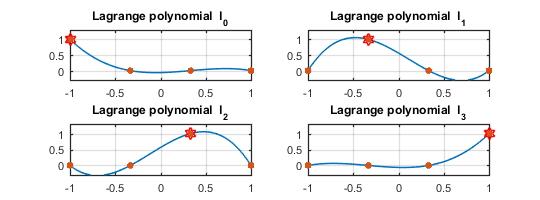
\includegraphics [width=4in]{chap15_01.png}
\begin{par}
 \vskip 1pt 
\end{par} \vspace{1em}
\begin{par}
By taking the absolute values of these curves, we see the largest possible effect at each point in $[-1,1]$ of data that is nonzero at just one point of the grid:
\end{par} \vspace{1em}
\begin{par}
 \vskip -2em 
\end{par} \vspace{1em}
\begin{verbatim}
for k = 1:npts
  subplot(2,2,k), absp = abs(p{k});
  hold off, plot(absp), grid on, hold on, plot(s,absp(s),'.')
  plot(s(k),absp(s(k)),'hr','markersize',9), ylim([-.3 1.3])
  title(['Absolute value  |l_' int2str(k-1) '(x)|'],FS,9)
end
\end{verbatim}

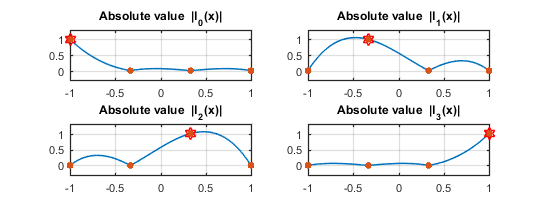
\includegraphics [width=4in]{chap15_02.png}
\begin{par}
 \vskip 1pt 
\end{par} \vspace{1em}
\begin{par}
Now let us add up these absolute values as in (15.3):
\end{par} \vspace{1em}
\begin{par}
 \vskip -2em 
\end{par} \vspace{1em}
\begin{verbatim}
x = chebfun('x'); L = 0*x;
for k = 1:npts, L = L + abs(p{k}); end
clf, plot(L), grid on, hold on, plot(s,L(s),'.')
axis([-1 1 0 2])
title('Lebesgue function \lambda(x) for 4 equispaced points',FS,9)
\end{verbatim}

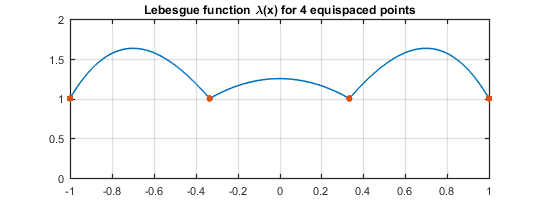
\includegraphics [width=4in]{chap15_03.png}
\begin{par}
 \vskip 1pt 
\end{par} \vspace{1em}
\begin{par}
This is the Lebesgue function $\lambda(x)$, a piecewise polynomial, telling us the largest possible effect at each point $x\in [-1,1]$ of interpolating data of norm 1. The Lebesgue constant (15.4) is the height of the curve:
\end{par} \vspace{1em}
\begin{par}
 \vskip -2em 
\end{par} \vspace{1em}
\begin{verbatim}
Lconst = norm(L,inf)
\end{verbatim}

        \color{lightgray} \begin{verbatim}Lconst =
   1.631130309440899
\end{verbatim} \color{black}
    \begin{par}
A code \texttt{lebesgue} for automating the above computation (actually based on a more efficient method) is included in Chebfun, and it optionally returns the Lebesgue constant as well as the Lebesgue function. Here are the results for 8 equispaced points:
\end{par} \vspace{1em}
\begin{par}
 \vskip -2em 
\end{par} \vspace{1em}
\begin{verbatim}
s = linspace(-1,1,8); [L,Lconst] = lebesgue(s);
hold off, plot(L), grid on, hold on, plot(s,L(s),'.')
title('Lebesgue function for 8 equispaced points',FS,9), Lconst
axis([-1 1 0 8])
\end{verbatim}

        \color{lightgray} \begin{verbatim}Lconst =
   6.929739656126463
\end{verbatim} \color{black}
    
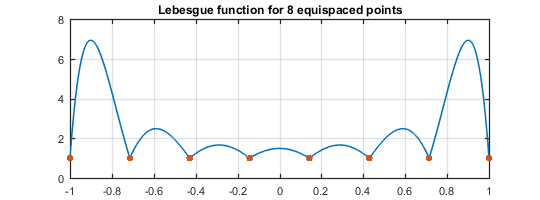
\includegraphics [width=4in]{chap15_04.png}
\begin{par}
 \vskip 1pt 
\end{par} \vspace{1em}
\begin{par}
And here they are for 12 points.  Note that the Lebesgue constant has jumped from 7 to 51.
\end{par} \vspace{1em}
\begin{par}
 \vskip -2em 
\end{par} \vspace{1em}
\begin{verbatim}
s = linspace(-1,1,12); [L,Lconst] = lebesgue(s);
hold off, plot(L), grid on, hold on, plot(s,L(s),'.')
title('Lebesgue function for 12 equispaced points',FS,9), Lconst
\end{verbatim}

        \color{lightgray} \begin{verbatim}Lconst =
  51.214223185730248
\end{verbatim} \color{black}
    
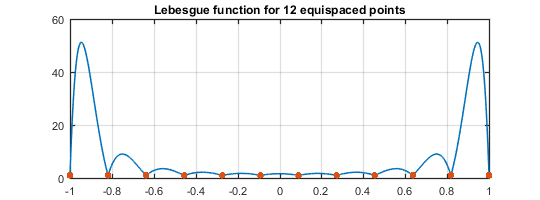
\includegraphics [width=4in]{chap15_05.png}
\begin{par}
 \vskip 1pt 
\end{par} \vspace{1em}
\begin{par}
The function takes large values near $\pm 1$, as we expect from Chapter 13 since the Runge phenomenon is associated with interpolants becoming very large near the endpoints.  In fact the Lebesgue function for interpolation in equispaced points is more naturally displayed on a log scale.  Here it is for $n=30$:
\end{par} \vspace{1em}
\begin{par}
 \vskip -2em 
\end{par} \vspace{1em}
\begin{verbatim}
s = linspace(-1,1,30); [L,Lconst] = lebesgue(s);
hold off, semilogy(L), grid on, hold on, semilogy(s,L(s),'.')
title('Lebesgue function for 30 equispaced points',FS,9)
Lconst
\end{verbatim}

        \color{lightgray} \begin{verbatim}Lconst =
     3.447738672845218e+06
\end{verbatim} \color{black}
    
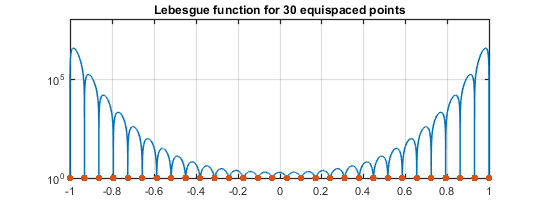
\includegraphics [width=4in]{chap15_06.png}
\begin{par}
 \vskip 1pt 
\end{par} \vspace{1em}
\begin{par}
For comparison, here are the corresponding results for 4, 8, and 12 Chebyshev points, now back again on a linear scale.
\end{par} \vspace{1em}
\begin{par}
 \vskip -2em 
\end{par} \vspace{1em}
\begin{verbatim}
for npts = 4:4:12
  s = chebpts(npts); [L,Lconst] = lebesgue(s);
  hold off, plot(L), grid on, hold on, plot(s,L(s),'.')
  title(['Lebesgue function for ' int2str(npts) ' Chebyshev points'],FS,9)
  axis([-1 1 0 3])
  snapnow, Lconst
end
\end{verbatim}

        \color{lightgray} \begin{verbatim}Lconst =
   1.666666666666667
\end{verbatim} \color{black}
    
        \color{lightgray} \begin{verbatim}Lconst =
   2.202214555205529
\end{verbatim} \color{black}
    
        \color{lightgray} \begin{verbatim}Lconst =
   2.489430376881967
\end{verbatim} \color{black}
    
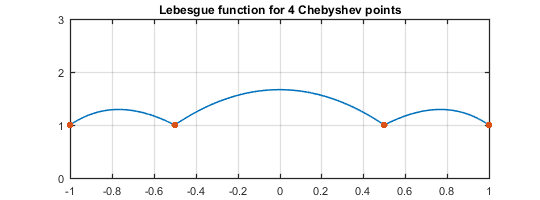
\includegraphics [width=4in]{chap15_07.png}

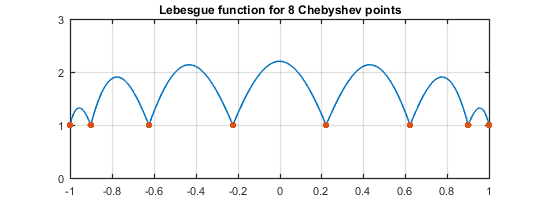
\includegraphics [width=4in]{chap15_08.png}

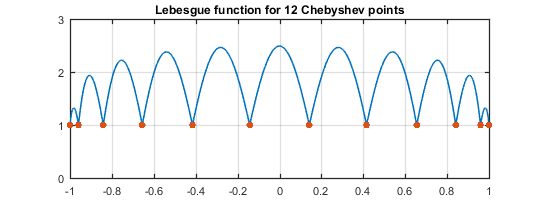
\includegraphics [width=4in]{chap15_09.png}
\begin{par}
 \vskip 1pt 
\end{par} \vspace{1em}
\begin{par}
Here are 100 Chebyshev points, with a comparison of the actual Lebesgue constant with the bound from Theorem 15.2:
\end{par} \vspace{1em}
\begin{par}
 \vskip -2em 
\end{par} \vspace{1em}
\begin{verbatim}
npts = 100; s = chebpts(npts); [L,Lconst] = lebesgue(s);
clf, plot(L,'linewidth',0.7), grid on, ylim([0 5])
Lconst, Lbound = 1 + (2/pi)*log(npts)
title('Lebesgue function for 100 Chebyshev points',FS,9)
\end{verbatim}

        \color{lightgray} \begin{verbatim}Lconst =
   3.887871431579912
Lbound =
   3.931742395517711
\end{verbatim} \color{black}
    
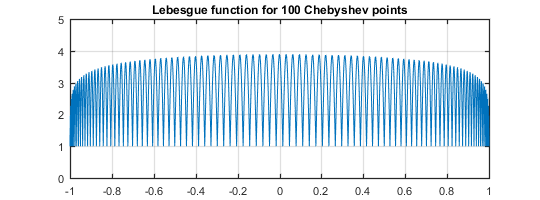
\includegraphics [width=4in]{chap15_10.png}
\begin{par}
 \vskip 1pt 
\end{par} \vspace{1em}
\begin{par}
The low height of this curve shows how stable Chebyshev interpolation is.
\end{par} \vspace{1em}
\begin{par}
In Chapter 9 it was mentioned that combinations of Lagrange polynomials can explain both the Gibbs phenomenon and the size of Lebesgue functions. Let us now explain this remark.  To analyze the Gibbs oscillations near a step, we added up a succession of Lagrange polynomials with constant amplitude $1$.  Since a single Lagrange polynomial has an oscillatory inverse-linear tail, the sum corresponds to an alternating series that converges as $n\to\infty$ to a constant. Lebesgue functions, on the other hand, are defined by taking a \textit{maximum} at each point on the grid.  The maximum is achieved by adding up Lagrange polynomials with equal but alternating coefficients, so as to make the combined signs all equal. For example, on the 20-point Chebyshev grid, the maximum possible value of an interpolant is achieved at $x=0$ by taking data with this pattern:
\end{par} \vspace{1em}
\begin{par}
 \vskip -2em 
\end{par} \vspace{1em}
\begin{verbatim}
s = chebpts(20); d = (-1).^[1:10 10:19]';
plot(s,d,'.k'), ylim([-2.5 3.5])
title('Worst possible data for Chebyshev interpolant',FS,9)
\end{verbatim}

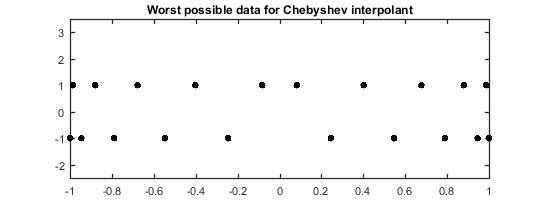
\includegraphics [width=4in]{chap15_11.png}
\begin{par}
 \vskip 1pt 
\end{par} \vspace{1em}
\begin{par}
Here is the Chebyshev interpolant:
\end{par} \vspace{1em}
\begin{par}
 \vskip -2em 
\end{par} \vspace{1em}
\begin{verbatim}
p = chebfun(d);
hold on, plot(p)
title('Interpolant through worst possible data',FS,9)
\end{verbatim}

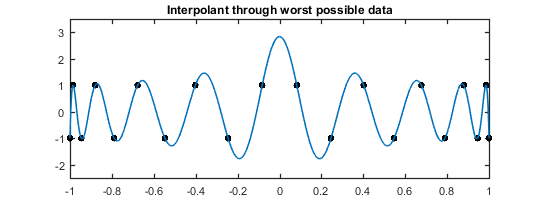
\includegraphics [width=4in]{chap15_12.png}
\begin{par}
 \vskip 1pt 
\end{par} \vspace{1em}
\begin{par}
We readily confirm that the maximum of this interpolant is indeed the Lebesgue constant for this grid:
\end{par} \vspace{1em}
\begin{par}
 \vskip -2em 
\end{par} \vspace{1em}
\begin{verbatim}
max(p)
[L,Lconst] = lebesgue(s);
Lconst
\end{verbatim}

        \color{lightgray} \begin{verbatim}ans =
   2.837131699740444
Lconst =
   2.837131699740441
\end{verbatim} \color{black}
    \begin{par}
We can now summarize why Lebesgue constants for Chebyshev points, and indeed for any sets of interpolation points, must grow at least logarithmically with $n.$  The fastest a Lagrange polynomial can decay is inverse-linearly, and the Lebesque function adds up those alternating tails with alternating coefficients, giving a harmonic series.
\end{par} \vspace{1em}
\begin{par}
Our discussion in this chapter has focussed on Chebyshev interpolation rather than projection.  However, as usual, there are parallel results for projection, which historically were worked out earlier (for the Fourier case, not Chebyshev). We record here a theorem analogous to Theorem 15.2.
\end{par} \vspace{1em}
\begin{par}
 \em
{\bf Theorem 15.3.  Lebesgue constants for Chebyshev projection.}
The Lebesgue constants $\Lambda_n$ for degree $n\ge 1$
Chebyshev projection in $[-1,1]$ are given by
$$ \Lambda_n = {1\over 2\pi} \int_{-\pi}^\pi \left|
{\sin((n+1/2) t)\over \sin(t/2)}\right| \, dt. \eqno (15.10) $$
They satisfy
$$ \Lambda_n\le {4\over\pi^2}\log (n+1) + 3~~~~and~~~~
\Lambda_n\sim{4\over\pi^2}\log n, ~~n\to\infty. \eqno (15.11a,b) $$
\vspace{-1.5em} 
\end{par} \vspace{1em}
\begin{par}
\textit{Proof.} See [Rivlin 1981].  Equation (15.11b) is due to $\hbox{Fej\'er}$ in 1910 $\hbox{[Fej\'er}$ 1910]. $~\hbox{\vrule width 2.5pt depth 2.5 pt height 3.5 pt}$
\end{par} \vspace{1em}
\begin{par}
Related to Theorem 15.3 is another result concerning the norm of projection operators, proved by Landau [1913]. If $f$ is analytic in the unit disk and continuous on the boundary, and $p\in {\cal P}_n$ is the \textit{Taylor projection} of $f$ obtained by truncating its Taylor series, how much bigger can $p$ be than $f$ on the unit disk?  Landau showed that these norms (now known as \textit{Landau constants}) grow at a rate asymptotic to $(1/\pi) \log n$ as $n\to\infty$, a discovery that is perhaps the starting point of all results about logarithmic growth of norms of approximation operators.
\end{par} \vspace{1em}
\begin{par}
For details about Lebesgue constants, an outstanding source is the survey article by Brutman [1997].
\end{par} \vspace{1em}
\begin{par}

\begin{displaymath}
\framebox[4.7in][c]{\parbox{4.5in}{\vspace{2pt}\sl
{\sc Summary of Chapter 15.}
The Lebesgue constant for interpolation or any other linear projection is
the $\infty$-norm of the operator mapping data to approximant. For interpolation in
$n+1$ Chebyshev points the Lebesgue constant is bounded by $1 +
2\pi^{-1}\log(n+1)$, whereas for $n+1$ equispaced points it is asymptotic
to $2^{n+1}/e\kern .7pt n \kern .7pt \log(n)$.\vspace{2pt}}}
\end{displaymath}

\end{par} \vspace{1em}
\begin{par}
 \smallskip\small\parskip=2pt
{\bf Exercise 15.1. Plots of Lebesgue functions.} Plot the Lebesgue
functions for the following distributions of interpolation points.
(a) $-0.9$, $-0.8$, $0$, $0.1$, $0.2$, $0.8$.
(b) Same as in (a) but with additional points at a distance $0.01$ to the
right of the others.
\par
{\bf Exercise 15.2.  Chebyshev points of the first kind.} The Lebesgue
constants for degree $n$ Chebyshev interpolation are bounded by those for
degree $n$ interpolation in Chebyshev points of the first kind,
introduced in Exercise 2.4 (see also \verb|help chebpts|),
with equality when $n$ is odd (Ehlich and Zeller
[1966], McCabe and Phillips [1973]). Verify this numerically for $0\le n
\le 20$.
\par
{\bf Exercise 15.3.  Reproducing a table by Brutman.} Page 698 of
[Brutman 1978] gives a table of various quantities associated with the
Lebesgue function for interpolation in Chebyshev points of the first
kind, mentioned in the last exercise.
Track down this paper and write the shortest, most elegant Chebfun
program you can to duplicate this table. Are all of Brutman's digits
correct?
\par
{\bf Exercise 15.4.  Omitting the endpoints.} Suppose one performs
polynomial interpolation in the usual Chebyshev points (2.2), but
omitting the endpoints $x=\pm 1$. Perform numerical experiments to
determine what happens to the Lebesgue constants in this case.  Does the
growth appear to still be of order $\log n$, or $n^\alpha$ for some
$\alpha$, or what?
\par
{\bf Exercise 15.5.  Optimal interpolation points.} Starting from the
$n+1$ Chebyshev points, one could attempt to use one of Matlab's
optimization codes to adjust the points to minimize the Lebesque
constant.  Do this and give the Lebesgue constant and plot the Lebesgue
function for (a) $n=4$, (b) $n=5$, (c) $n=6$, (d) $n=7$, and (e) $n=8$.
How much improvement do you find in the Lebesgue constants as compared
with Chebyshev points?
\par
{\bf Exercise 15.6.  Improving Turetskii's estimate.} For interpolation
in equispaced points, $\hbox{Sch\"onhage}$ [1961] derived a more accurate
estimate than (15.9b): $\Lambda_n\sim 2^{n+1}/e\kern 1pt n(\log n +
\gamma)$, where $\gamma = 0.577\dots$ is again Euler's constant. Perform
a numerical study of $\Lambda_n$ as a function of $n$ and see what
difference this correction makes.  For example, it might be helpful to
have a table showing the percentage errors in both estimates as functions
of $n$.
\par
{\bf Exercise 15.7.  Interpolating data with a gap.}
(a) Consider polynomial interpolation in $n+1$ points of a function $f$
defined on $[-1,1]$, with half the points equally spaced from $-1$ to
$-1/4$ and the other half equally spaced from $1/4$ to $1$.  Determine
the Lebesgue constants for this interpolation process numerically for the
cases $n+1 = 20$ and $40$.
(b) Suppose $f$ is analytic and bounded by $1$ in the $\rho$-ellipse
$E_\rho$ with $\rho=2$.  Carefully quoting theorems from this book as
appropriate, give upper bounds for the error $|f(0)-p(0)|$ for these two
cases.
\par
{\bf Exercise 15.8.  Smallest local minimum of the Lebesgue function.}
Interpolation in equispaced points is much better near the middle of an
interval than at the ends.  In particular, the smallest local maximum of
the Lebesgue function $\lambda$ is $\sim \log n / \pi$ as $n\to\infty$
[Tietze 1917]. Make a plot of these minima as a function of $n$ to verify
this behavior numerically.
\par
{\bf Exercise 15.9.  Convergence for Weierstrass's function.}
Exercise 7.3 promised that in Chapter 15, we would show that Chebyshev
interpolants to Weierstrass's nowhere-differentiable function of Exercise
6.1 converge as $n\to\infty$.  Write down such a proof based on combining
various theorems of this book.
\par
{\bf Exercise 15.10. Random interpolation points.}
(a) Compute Lebesgue functions and constants numerically for degree $n$
interpolation in uniformly distributed random points in $[-1,1]$.  How
does $\Lambda$ appear to grow with $n$?
(b) Same question for points randomly distributed according to the
Chebyshev density (11.18).
\par
{\bf Exercise 15.11.  A wiggly function.}  (a) Let $f$ be the function
$T_{m}(x) + T_{m+1}(x) + \cdots + T_{n}(x)$ with $m=20$ and $n=40$, and
let $p^*$ be the best approximation of $f$ of degree $m-1$.  Plot $f$ and
$f-p^*$.  What are their $\infty$-norms and $2$-norms?  (b) The same
questions with $m=200$ and $n=300$.
\par
{\bf Exercise 15.12.  Divergence of Lebesgue constants.} Spell out precisely the
reasoning used to justify (15.6) in the text.  In particular,
make it clear why a ``$\limsup$'' rather than a ``$\sup$'' appears
in the formula.
\par
{\bf Exercise 15.13.  Confluent interpolation nodes.}
Let $\{x_j\}$ be a set of $n+1$ distinct interpolation nodes in $[-1,1]$.
Now change $x_0$ to $x_1+\varepsilon$,
where $\varepsilon>0$ is a parameter, and let
$\Lambda(\varepsilon)$ be the corresponding Lebesgue constant.  Show that
$\Lambda(\varepsilon)$ diverges to $\infty$ as $\varepsilon\to 0$.  Can you
quantify the rate of divergence?
\par 
\end{par} \vspace{1em}



\end{document}
    
